\documentclass{article}
\usepackage{geometry}
\usepackage{listings}
\usepackage{textcomp}
\usepackage{graphicx}
\usepackage[hidelinks]{hyperref}
\usepackage{hyperref}
\usepackage{appendix}
\usepackage{multirow}
\usepackage{amsmath,amssymb,amsfonts}
\usepackage[framed,numbered,autolinebreaks,useliterate]{mcode}
%记得用xelatex
% 导入首行缩进用的宏包
\usepackage{indentfirst}
\setlength{\parindent}{2em}
% 每行缩进两个汉字
\usepackage{url}
\setlength{\parindent}{0pt}
\setlength{\parskip}{18pt}
\title{\vspace{+4cm}\textbf{Second Applied Mathematics Assignment}}
\author{Jianqi Feng 202023092020}
\date{\today}
% //////////////////////////////////////////////////

\begin{document}
%标题
\maketitle
%目录
\newpage
\pagenumbering{Roman}
\setcounter{page}{0}
\tableofcontents

\newpage
\setcounter{page}{1}
\pagenumbering{arabic}
\setlength{\parindent}{2em}

\section{Newton’s interpolatory polynomial}
\subsection{Background of the method}
Suppose that $P_{n}(x)$ is the nth Lagrange polynomial that agrees with the function $f$ at
the distinct numbers $x_0$, $x_1$,..., $x_n$. The divided differences of $f$
with respect to $x_0$, $x_1$,..., $x_n$ are used to express $P_{n}(x)$ in the form

\begin{align}
P_{n}(x) = a_0 + a_1(x - x_0) + a_2(x - x_0)(x - x_1) +...+ a_n(x - x_0)...(x - x_{n-1})
\label{P1}
\end{align}

Then we could input the points to (\ref{P1}) and solve $a_0$, $a_1$,..., $a_n$ as follows

\begin{align}
a_0 = P_{n}(x_0) = f (x_0) \quad ,\quad a_1 = \frac{f (x_1) - f (x_0)}{x_1 - x_0}\nonumber 
\end{align}

If define $ f [x_i, x_{i+1}] = \frac{f [x_{i+1}] - f [x_i]}{x_{i+1} - x_i}$ ,then we can get

\begin{align}
f [x_i, x_{i+1},..., x_{i+k−1}, x_{i+k} ] = \frac{f [x_{i+1}, x_{i+2},..., x_{i+k} ] - f [x_{i}, x_{i+1},..., x_{i+k−1}]}{x_{i+k} - x_i}\nonumber 
\end{align}


And that $a_n = f [x_0, x_1,..., x_{n-1}, x_{n}]$ , so we could get a form without $a_n$ ,which we called Newton's Divided-Difference:
\begin{align}
P_{n}(x) = f [x_0] +\sum_{k=1}^n
f[x_0, x_1,..., x_k]\prod_{i=0}^{k-1}(x - x_i)
\label{P2}
\end{align}


Then we could calculate the $f [x_0, x_1,..., x_{n-1}, x_{n}]$ like shown in the table as follow:

%插入图片
\begin{figure}[h!]
\centering
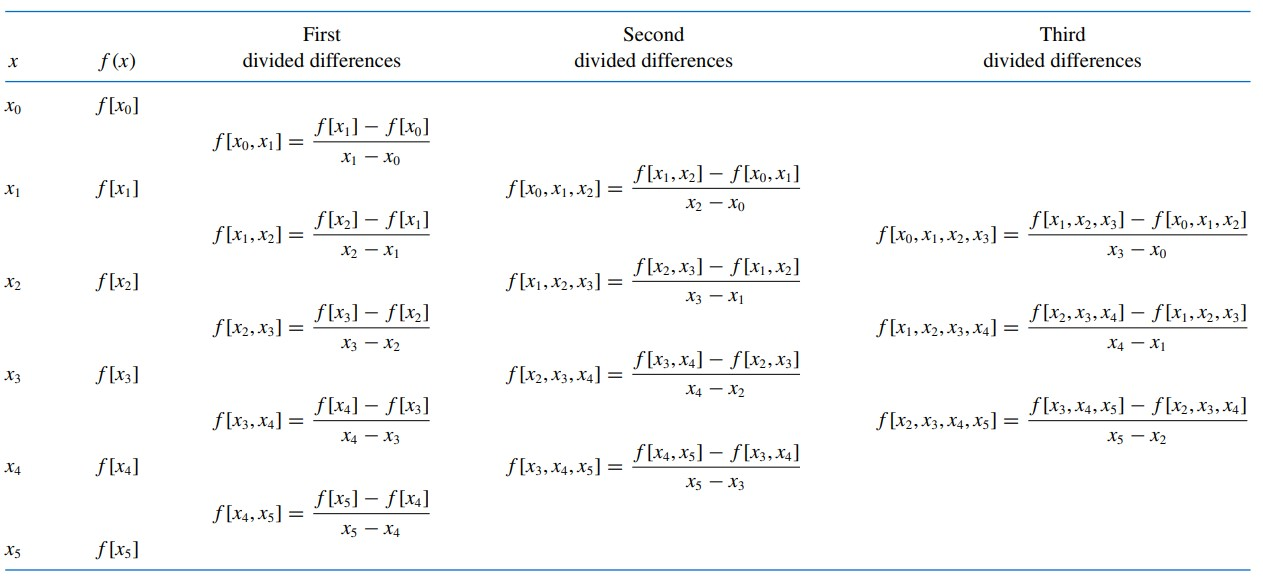
\includegraphics[width=1\textwidth]{newton1.JPG}
\caption{Newton’s Divided-Difference Formula}
\label{newton1}
\end{figure}

\newpage
\subsection{Code of Newton's method}

According to (\ref{P2}) , we could get the code in Matlab to make Newton’s interpolatory polynomial come true

\begin{lstlisting}
%Newton's interpolatory polynomial
clc;clear;
format long
% Part1 : Input the numbers and the values
x = [1.0
    1.3
    1.6
    1.9
    2.2]; %numbers
f = [0.7651977
    0.6200860
    0.4554022
    0.2818186
    0.1103623]; %values

%Part2 : Calculate the Divided differences
n = length(x);
A = [ x , f , zeros(n,n-1) ];
for j = 3 : (n+1)
    for i = 1 : n+2-j
        A(i,j) = ( A(i+1,j-1) - A(i,j-1) ) / (A(i+j-2,1)-A(i,1));
    end
end
A % Show the divided differences

%Part3 : Calculate the Polynomial
%Draw the function
t = linspace( x(1) , x(n) , 100);
y = zeros( 1 , length(t) );
for m = 1 : length(t)
    p = f(1);
    g = 1;
    for k = 1 : n-1
    g = g * ( t(m) - x(k) );
    p = p + A(1,k+2) * g;
    end
    y(m) = p ;
end
plot(t,y,x,f,'o');
% We can also get the function as flow
% syms t
% p = f(1);
% g = 1;
% for k = 1 : n-1
%     g = g * ( t - x(k) );
%     p = p + A(1,k+2) * g;
% end
% p
\end{lstlisting}

Then we input the numbers in Example 1 and get the same results which shows that the code is correct.


\section{Pieceise Hermite interpolatory polynomial}
\subsection{Background of the method}
Based on the Newton's method,if we also get the values of $f'$,we could improve the Newton's method by add the $ f [x_i, x_i] = f'(x_i)$.Suppose that the distinct numbers $x_0$, $x_1$,..., $x_n$ are given together with the values of
$f$ and $f'$ at these numbers. Define a new sequence $z_0$,$z_1$,...,$z_{2n+1}$ by

\begin{align}
z_{2i} = z_{2i+1} = x_i,\quad \mbox{for each} \ i = 0, 1, ... , n\nonumber
\end{align}

Based on the Newton's method we define $f[z_{2i},z_{2i+1}] = f'(z_{2i}) = f (x_i) $,then we could get the Hermite polynomial as follows

\begin{align}
H_{2n+1}(x) = f [z_0] + \sum_{k=1}^{2n+1}f[z_0,...,z_k ]\prod_{i=0}^{k-1}(x - z_i)
\label{hermite1}
\end{align}


We could calculate the $f [z_0, z_1,..., z_{n-1}, z_{n}]$ like shown in the table as follow:

\begin{figure}[h!]
\centering
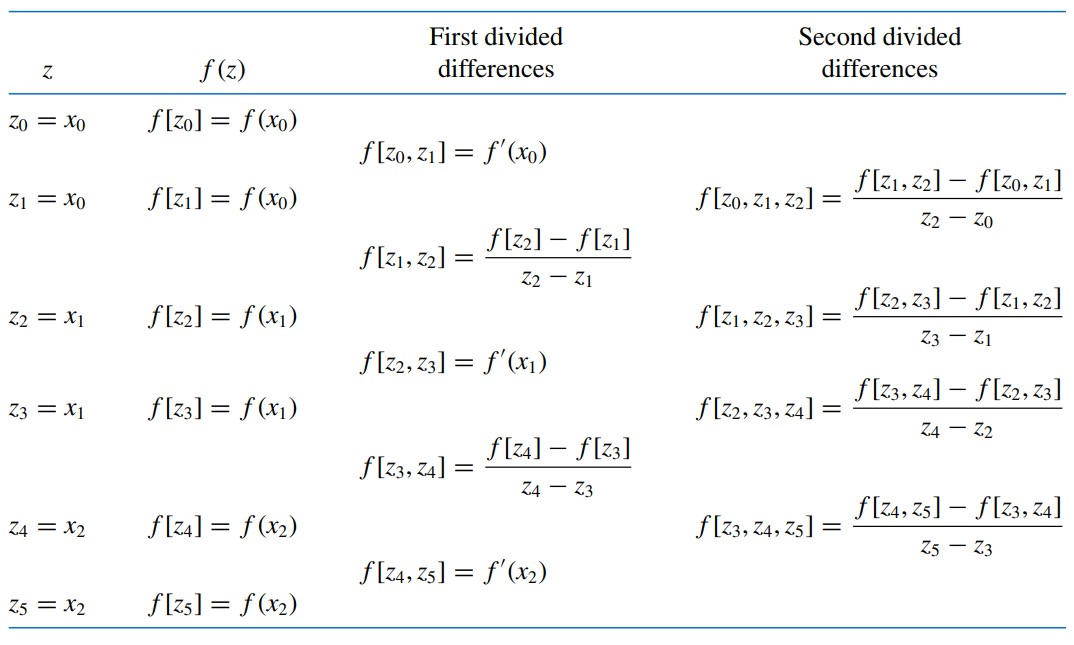
\includegraphics[width=1\textwidth]{hermite1.JPG}
\caption{Hermite interpolatory polynomial}
\label{hermite1}
\end{figure}

\subsection{Code of Hermite's method}


According to (\ref{hermite1}) , we could get the code in Matlab to make Hermite interpolatory polynomial come true

\begin{lstlisting}
%Hermite interpolatory polynomial
clc;clear;
format long
%Part1 : Input the points
x = [1.3
    1.6
    1.9]; %numbers
f = [0.6200860
    0.4554022
    0.2818186]; %values
df = [-0.5220232
    -0.5698959
    -0.5811571]; %diff

%Part2 : Calculate the Matrix
n = length( x );
Q = zeros( 2*n , 2*n );
z = zeros( 1 , 2*n );
for i = 1 : n
    z( 2 * i - 1 ) = x( i );
    z( 2 * i ) = x( i );
    Q( 2 * i - 1 , 1 ) = f( i );
    Q( 2 * i , 1 ) = f( i );
    Q( 2 * i - 1, 2 ) = df( i );
    if i ~= 1
        Q( 2 * (i-1) , 2) = ( Q(2*i-1,1)-Q(2*(i-1),1) )/( x(i)-x(i-1) );
    end
end
for j = 3 : 2*n
    for i = 1 : 2*n+1-j
        Q(i,j)=( Q(i+1,j-1)-Q(i,j-1) )/( z(i+j-1)-z(i) );
    end
end

%Part3 : Draw the polynomial
t = linspace( x(1) , x(n) , 100);
y = zeros( 1 , length(t) );
for m = 1 : length(t)
    p = f(1);
    g = 1;
    for k = 2 : 2*n
    g = g * ( t(m) - z(k-1) );
    p = p + Q(1,k) * g;
    end
    y(m) = p ;
end
plot(t,y,x,f,'o');
\end{lstlisting}

We input the numbers in Example 1 and get the same results which shows that the code is correct.


\subsection{Pieceise Hermite interpolatory}

If the values of $f$ and of $f'$ are known at each of the points $x_0 < x_1 < ... < x_n$, a cubic
Hermite polynomial can be used on each of the subintervals $[x_0, x_1]$, $[x_1, x_2]$,..., $[x_{n−1}, x_n]$
to obtain a function that has a continuous derivative on the interval $[x_0, x_n]$

Then we could get the code of Pieceise Hermite interpolatory by the function in Matlab as follows

\begin{lstlisting}
%Piecewise Hermite interpolatory polynomial
clc;clear;
format long
%Part1 : Input the points
x = [1.3
    1.6
    1.9]; %numbers
f = [0.6200860
    0.4554022
    0.2818186]; %values
df = [-0.5220232
    -0.5698959
    -0.5811571]; %diff
n = length(x);

%Part2 : Piecewise Hermite
t = linspace(x(1),x(n),100);
y = [f(1)];
for i = 1:n-1
    s = t(t<=x(i+1) & t>x(i));
    y0 = hermite( [x(i),x(i+1)] , [f(i),f(i+1)] , [df(i),df(i+1)] , 0 , s );
    y = [y,y0];
end

%Part3 : Compare the polynomial
y1 = hermite(x,f,df,0,t); % donot piecewise
plot(t,y1,t,y);
legend('Without Piecewise','With Piecewise');
title('Compare of the two methods');
xlabel('x');
ylabel('f(x)');
plot(t,y1-y); %compare the difference
title('Difference of the two methods');
xlabel('x');
ylabel('f1(x)-f2(x)');

function y0 = hermite(xx,ff,dff,p,s)
%Piecewise Hermite interpolatory polynomial
format long
%Part1 : Input the points
x = xx; %numbers
f = ff; %values
df = dff; %diff

%Part2 : Calculate the Matrix
n = length( x );
Q = zeros( 2*n , 2*n );
z = zeros( 1 , 2*n );
for i = 1 : n
    z( 2 * i - 1 ) = x( i );
    z( 2 * i ) = x( i );
    Q( 2 * i - 1 , 1 ) = f( i );
    Q( 2 * i , 1 ) = f( i );
    Q( 2 * i - 1, 2 ) = df( i );
    if i ~= 1
        Q( 2 * (i-1) , 2) = ( Q(2*i-1,1)-Q(2*(i-1),1) )/( x(i)-x(i-1) );
    end
end
for j = 3 : 2*n
    for i = 1 : 2*n+1-j
        Q(i,j)=( Q(i+1,j-1)-Q(i,j-1) )/( z(i+j-1)-z(i) );
    end
end

%Part3 : Draw the polynomial
t = linspace(x(1),x(n),p);
t = s ;
y0 = zeros( 1 , length(t) );
for m = 1 : length(t)
    p = f(1);
    g = 1;
    for k = 2 : 2*n
    g = g * ( t(m) - z(k-1) );
    p = p + Q(1,k) * g;
    end
    y0(m) = p ;
end
end
\end{lstlisting}

Then we could compare and get the difference between Pieceise Hermite interpolatory and Hermite interpolatory as follows

\begin{figure}[htbp]
\centering
\subfigure{
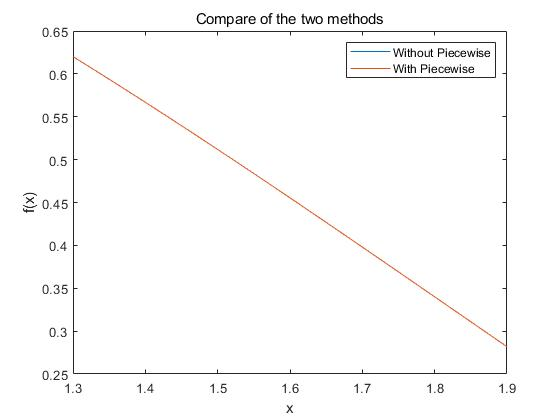
\includegraphics[width=7cm]{hermite2.jpg}
}
\quad
\quad
\subfigure{
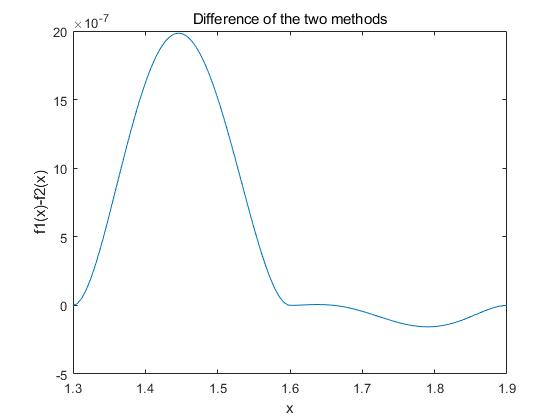
\includegraphics[width=7cm]{hermite3.jpg}
}
\caption{Difference before and after piecewise}
\end{figure}


\section{Natural Splines interpolatory polynomial}
\subsection{Background of the method}
A spline defined on an interval that is divided into $n$
subintervals will require determining 4n constants. To construct the cubic spline interpolant
for a given function $f$ , the conditions in the definition are applied to the cubic polynomials

\begin{align}
S_{j}(x) = a_j + b_{j}(x - x_j) + c_{j}(x - x_j)^2 + d_{j}(x - x_j)^3\nonumber
\label{taylor1}
\end{align}

for each $j = 0, 1,..., n - 1$.We have the condition as follow

\begin{equation}
    \begin{cases}
        S_{j}(x_j) = a_j = f (x_j) \\
        S_{j+1}(x_{j+1}) = S_{j}(x_{j+1})
     \end{cases}
\end{equation}

Solve this equation and we could get the equations as follow($h_j = x_{j+1} - x_j$),
\begin{align}
h_{j-1}c_{j-1} + 2(h_{j-1} + h_{j})c_j + h_{j}c_{j+1} = \frac{3}{h_j}(a_{j+1} - a_j) − \frac{3}{h_{j-1}}(a_j - a_{j-1})
\label{natural}
\end{align}

By the LU Factorization,we could solve the $a_j$,$b_j$,$c_j$,and $d_j$ (Theorem 6.21 in Section 6.6)

\subsection{Code of the method}
According to (\ref{natural}) , we could get the code in Matlab to make Hermite interpolatory polynomial come true

\begin{lstlisting}
%Natural Cubic Spline interpolatory polynomial
%Part1 : Input the numbers and the values
x = [0
    1
    2
    3]; %points
f = [1
    exp(1)
    exp(2)
    exp(3)]; %values
n = length(x);

%Part2 : Calculate the a,b,c,d
for i = 1 : n-1
    h(i) = x(i+1) - x(i);
end
for i = 2 : n-1
    a(i) = 3*( f(i+1) - f(i) )/h(i) - 3*( f(i) - f(i-1) )/h(i-1);
end
l = ones(1,n);
u = zeros(1,n);
z = zeros(1,n);
for i = 2 : n-1
    l(i) = 2*( x(i+1)-x(i-1) ) - h(i-1) * u(i-1);
    u(i) = h(i)/l(i);
    z(i) = (a(i)-h(i-1)*z(i-1))/l(i);
end
c = zeros(1,n);
b = zeros(1,n);
d = zeros(1,n);
for j = n-1:-1:1
    c(j) = z(j) - u(j)*c(j+1);
    b(j) = ( f(j+1)-f(j) )/h(j) - h(j)*( c(j+1)+2*c(j) )/3;
    d(j) = ( c(j+1)-c(j) )/(3*h(j));
end

%Part3 : Output the polynomial
t = linspace(x(1),x(n),100);
y = [f(1)];
for i = 1:n-1
    s = t(t<=x(i+1) & t>x(i));
    y0 = f(i) + b(i)*( s-x(i) ) + c(i)*( s-x(i) ).^2 + d(i)*( s-x(i) ).^3;
    y = [y,y0];
end
plot(t,y,t,exp(t));
legend('Polynomial','Function');
xlabel('x');
ylabel('f(x)');
title('Natural Cubic Spline')
\end{lstlisting}

We input the values in Example 2 and get the figure as follow which is as same as the results in the book,and it proves that the code is correct.
 
\begin{figure}[h!]
\centering
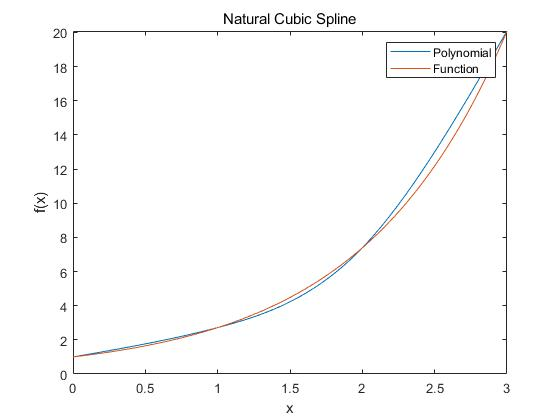
\includegraphics[width=0.7\textwidth]{natural.jpg}
\caption{Natural Cubic Spline of Example 2}
\label{hermite1}
\end{figure}
 
\newpage
\section{Compared the three methods}
When given the function $f(x)=\frac{5}{1+x^2}$,we take the points in 1l distinct over $[-5,5]$ and get the code as follow
\begin{lstlisting}
%Summary for Example
clc;clear;
x = (-5:5)';
n = length(x);
f = 5./(1 + x.^2);
df = -10.*x./(1 + x.^2).^2;
p = 100;

%Newton
y1 = newton(x,f,p);

%Piecewise Hermite
y2 = phermite(x,f,df,p);

%Natural
y3 = natural(x,f,p);

%Draw the figure
t = linspace(x(1),x(n),p);
y0 = 5./(1 + t.^2);
plot(t,y0,t,y1,t,y2,t,y3,x,f,'o');
legend('Function','Newton','Piecewise Hermite','Natural');
title('Polynomial of Different methods');
xlabel('x');
ylabel('f(x)');
\end{lstlisting}

And we could get the figure as follow

\begin{figure}[h!]
\centering
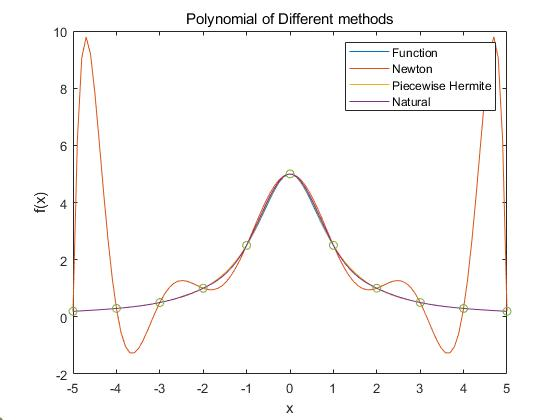
\includegraphics[width=0.6\textwidth]{summary.jpg}
\caption{Compared the three methods}
\label{summary}
\end{figure}
 
 In this figure we could see that the Newton's method has a strong Runge Phenomenon.According to the figures as follow ,we can also see that for this function,Piecewise Hermite has a better interpolatory ,followed by Natural Cubic Spline and the Newton's method is the worst.

\begin{figure}[htbp]
\centering
\subfigure{
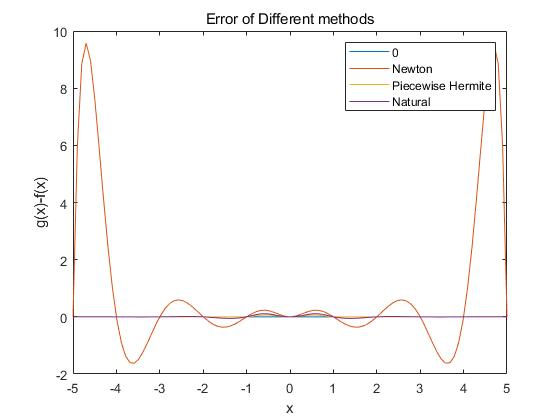
\includegraphics[width=7cm]{error.jpg}
}
\quad
\quad
\subfigure{
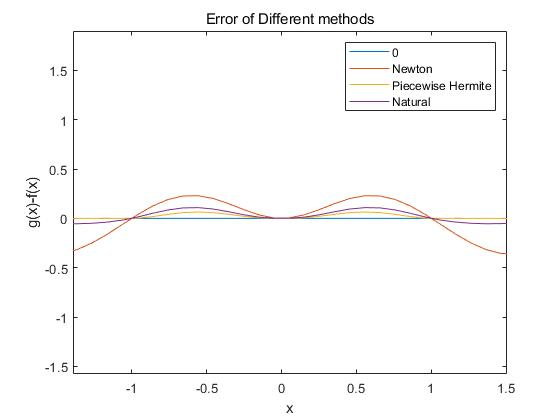
\includegraphics[width=7cm]{error2.jpg}
}
\caption{Error of the three methods}
\end{figure}

%参考文献
\newpage
\clearpage
\phantomsection
\addcontentsline{toc}{section}{References}
\tolerance=500
\begin{thebibliography}{99}  
\bibitem{ref1}Richard L. Burden, J. Douglas Faires, Annette M. Burden “Numerical Analysis” Cengage Learning, 2015
\end{thebibliography}

\newpage
\section*{Appendix}
\addcontentsline{toc}{section}{Appendix}
\subsection*{Function of Newton's method}
\lstinputlisting{newton.m}
\subsection*{Function of Hermite}
\lstinputlisting{hermite.m}
\subsection*{Function of Pieceise Hermite}
\lstinputlisting{phermite.m}
\subsection*{Function of Natural Splines}
\lstinputlisting{natural.m}
\end{document}





